\documentclass{article}

\usepackage[final]{style}
\usepackage[utf8]{inputenc} % allow utf-8 input
\usepackage[T1]{fontenc}    % use 8-bit T1 fonts
\usepackage{hyperref}       % hyperlinks
\usepackage{url}            % simple URL typesetting
\usepackage{booktabs}       % professional-quality tables
\usepackage{amsfonts}       % blackboard math symbols
\usepackage{nicefrac}       % compact symbols for 1/2, etc.
\usepackage{microtype}      % microtypography
\usepackage{verbatim}
\usepackage{graphicx}       % for figures
\usepackage{amsmath}
\usepackage[normalem]{ulem}
\usepackage{float}


\title{Lecture \#17: Motion}

\author{
  Kevin Chavez, Ben Cohen-Wang, Garrick Fernandez, Noah Jackson, Will Lauer \\
  Department of Computer Science\\
  Stanford University\\
  Stanford, CA 94305 \\
  \texttt{\{kechavez, bencw, garrick, noahjax, wlauer\}@cs.stanford.edu} \\
}

\begin{document}

\maketitle

\section{Introduction}
In this class so far we have learned a variety of tools that enable us to detect key points, recognize objects, and use segmentation in images. However, in many cases we want to be able to perform similar operations on video. Specifically, we are often interested not only in the location of certain objects, but also the movement of these objects over time. This lecture focuses on how we can apply previously covered techniques along with new methods to effectively track the motion of pixels across many images, with applications in areas such as self-driving cars, robots, and security systems to name a few.


\section{Optical Flow and Key Assumptions}

\subsection{Optical Flow}
Put simply, optical flow is the movement of pixels over time. The goal of optical flow is to generate a motion vector for each pixel in an image between $t_0$ and $t_1$ by looking at two images $I_0$ and $I_1$. By computing a motion vector field between each successive frame in a video, we can track the flow of objects, or, more accurately, "brightness patterns" over extended periods of time. However, it is important to note that while optical flow aims to represent the motion of image patterns, it is limited to representing the \textit{apparent} motion of these patterns. This nuanced difference is explained more in depth in the \textbf{Assumptions and Limitations} section. 

\subsection{Assumptions and Limitations}

\subsubsection{Apparent Motion}
Given a two dimensional image, optical flow can only represent the \textit{apparent} motion of brightness patterns, meaning that the movement vectors of optical flow can be the result of a variety of actions. For instance, variable lighting can cause strong motion vectors on static objects, and movement into or out of the frame cannot be captured by the 2D motion vectors of optical flow. One example of an issue poorly dealt with by  optical flow is the aperture problem. 

\begin{figure}[H]
\centering
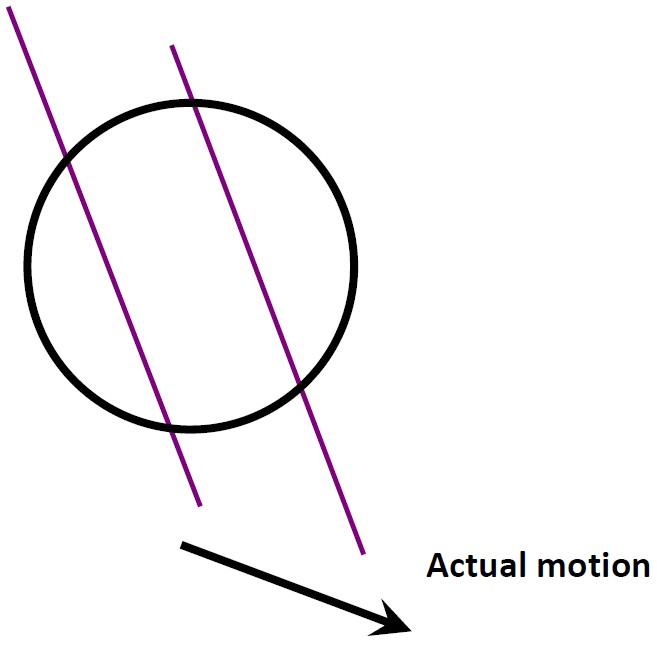
\includegraphics[width=6cm]{aperture-problem}
\caption{In the aperture problem, the line appears to have moved to the right when only in the context of the frame, but the true motion of the line was down and to the right. The aperture problem is a result of optical flow being unable to represent motion along an edge--an issue that can lead to other errors in motion estimation as well.}
\end{figure}

 

\subsubsection{Brightness Consistency}
As optical flow can only represent apparent motion, to correctly track the motion of points on an image we must assume that these points remain at the same brightness between frames. The equation for this brightness consistency equation is as follows
\[ I(x,y,t-1) = I(x+u(x,y), y+ v(x,y), t) \]
where u(x,y) represents the horizontal motion of a point and v(x,y) represents the vertical motion. 

\subsubsection{Small Motion}
Optical flow assumes that points do not move very far between consecutive images. This is often a safe assumption, as videos are typically comprised of 20+ frames per second, so motion between individual frames is small. However, in cases where the object is very fast or close to the camera this assumption can still prove to be untrue. To understand why this assumption is necessary, we must consider the \textbf{Brightness Consistency} equation defined above. When trying to solve this equation, it is useful to linearize the right side using a Taylor expansion. This yields
\[ I(x + u(x,y),y + v(x,y),t) \approx I(x,y,t-1) + I_x \cdot u(x,y) + I_y \cdot v(x,y) + I_t \]
Linearizing in this way allows us to solve for the u and v motion vectors we want, but in this case we have only included the first order Taylor series terms. When motion is large between frames, these terms do a poor job of capturing the entire motion, thus leading to inaccurate u,v. More information about higher order derivative constraints can be found in references [1], page 12.

\subsubsection{Spatial Coherence}
Spatial coherence is the assumption that nearby pixels will move together, typically because they are part of the same object. To see why this assumption is necessary, consider the equation for optical flow as defined above
\[ I(x + u(x,y),y + v(x,y),t) \approx I(x,y,t-1) + I_x \cdot u(x,y) + I_y \cdot v(x,y) + I_t \]
\[ I(x + u(x,y),y + v(x,y),t) - I(x,y,t-1) = I_x \cdot u(x,y) + I_y \cdot v(x,y) + I_t \]
Giving us 
\[I_x \cdot u + I_y \cdot v + I_t \approx 0 \]
\[ \bigtriangledown I \cdot [u \, v]^T + I_t = 0 \]
Ignoring the meaning of this derivation for the moment, it is clear that we do not have enough equations to find both u and v at every single pixel. Assuming that pixels move together allows us to use many more equations with the same [u v], making it possible to solve for the motion of pixels in this neighborhood.


\section{Lucas-Kanade}
Recovering image motion given by $(u,v)$ in the above equation requires at least two equations per pixel. To achieve this, the Lucas-Kanade \cite{lucas1981iterative} technique for image tracking relies on an additional constraint --- spatial coherence. 

The spatial coherence constraint is applied to a pixel using a window of size $k \times k$. The assumption is that the neighboring pixels in this window will have the same $(u,v)$. For example, in a $5x5$ window the following equations apply:
\[  0 = I_t(\mathbf{p_i}) + \nabla I(\mathbf{p_i}) \cdot [u \quad v] \]
\[ 
\begin{bmatrix}
	I_x(\mathbf{p_1}) & I_y(\mathbf{p_1}) \\
    I_x(\mathbf{p_2}) & I_y(\mathbf{p_2}) \\
    \vdots & \vdots \\
    I_x(\mathbf{p_{25}}) & I_y(\mathbf{p_{25}}) \\
\end{bmatrix}
\]
This produces an overly-constrained system of linear equations of the form $Ad=b$. Using a least squares method for solving over-constrained systems, we reduce the problem to solving for $d$ in $(A^TA)d=A^Tb$. More explicitly the system to solve is reduced to
\begin{align*}
\begin{bmatrix}
	\sum I_xI_x & \sum I_xI_y \\
    \sum I_yI_x & \sum I_yI_y
\end{bmatrix}&
\begin{bmatrix} u \\ v  \end{bmatrix} = 
- \begin{bmatrix} \sum I_xI_t \\ \sum I_yI_t \end{bmatrix} \\
A^TA \qquad \quad& \qquad \qquad \quad A^Tb
\end{align*}

\subsection{Condition for an Existing Solution}
In order to solve the system following conditions should hold:
\begin{itemize}
\item $A^TA$ should be invertible 
\item $A^TA$ should not be too small due to noise.
\subitem Eigenvalues $\lambda_1$ and $\lambda_2$ of $A^TA$ should not be too small 
\item $A^TA$ should be well-conditioned
\subitem i.e $\lambda_1 / \lambda_2$ should not be too large (for $\lambda_1 > \lambda_2$ )
\end{itemize}

\subsection{Geometric Interpretation}
It should be evident that the least squares system of equations above produce a second moment matrix $M = A^TA$. In fact, this is the Harris matrix for corner detection. 
\[ 
A^TA = 
\begin{bmatrix}
	\sum I_xI_x & \sum I_xI_y \\
    \sum I_yI_x & \sum I_yI_y
\end{bmatrix} = \sum
\begin{bmatrix} I_x \\ I_y \end{bmatrix} \begin{bmatrix} I_x & I_y \end{bmatrix} = \sum \nabla I ( \nabla I ) ^T = M
\]
We can relate the conditions above for solving the motion field $[u \quad v]$ to tracking corners detected by the Harris matrix $M$.  In particular, the eigenvectors and eigenvalues of $M=A^TA$ relate to the direction and magnitude of a possible edge in a region.  

Using this interpretation, it is apparent that an ideal region for Lucas-Kanade optical flow estimation is a corner. Visually, if $\lambda_1$ and $\lambda_2$ are too small this means the region is too “flat”.  If $\lambda_1 >> \lambda_2$, the method suffers from the aperture problem, and may fail to solve for correct optical flow.
\begin{figure}[H]
\centering
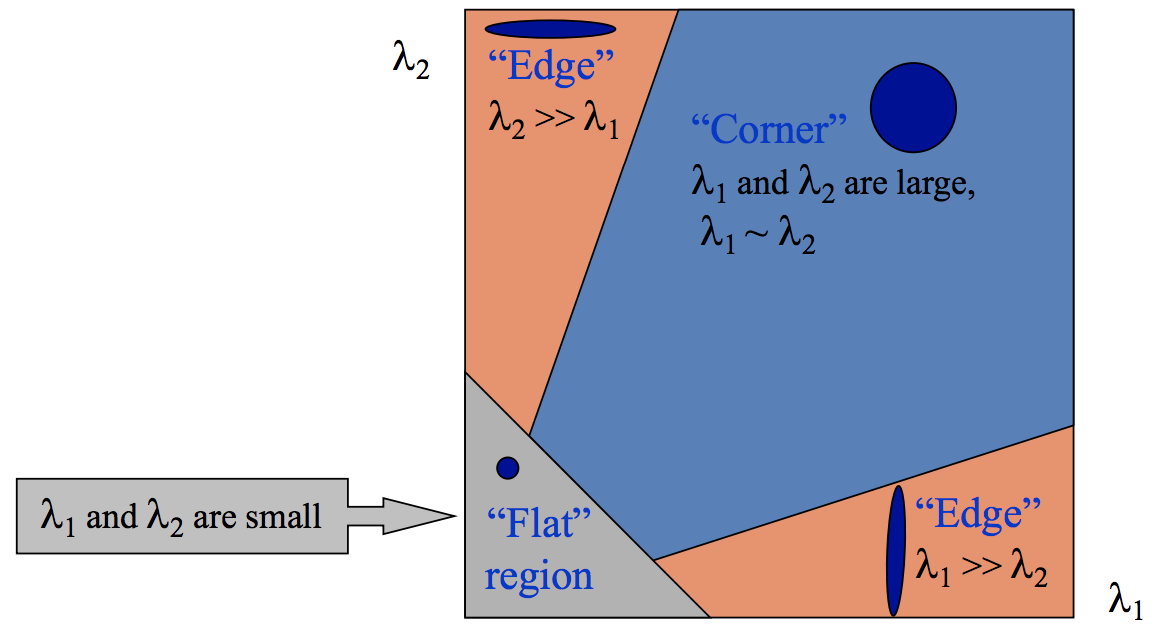
\includegraphics[width=\textwidth]{lk_eigen.png}
\caption{Conditions for a solvable matrix $A^TA$ may be interpreted as different edge regions depending on the relation between $\lambda_1$ and  $\lambda_2$. Corner regions produce more optimal conditions.}
\end{figure}

\begin{figure}[H]
\centering

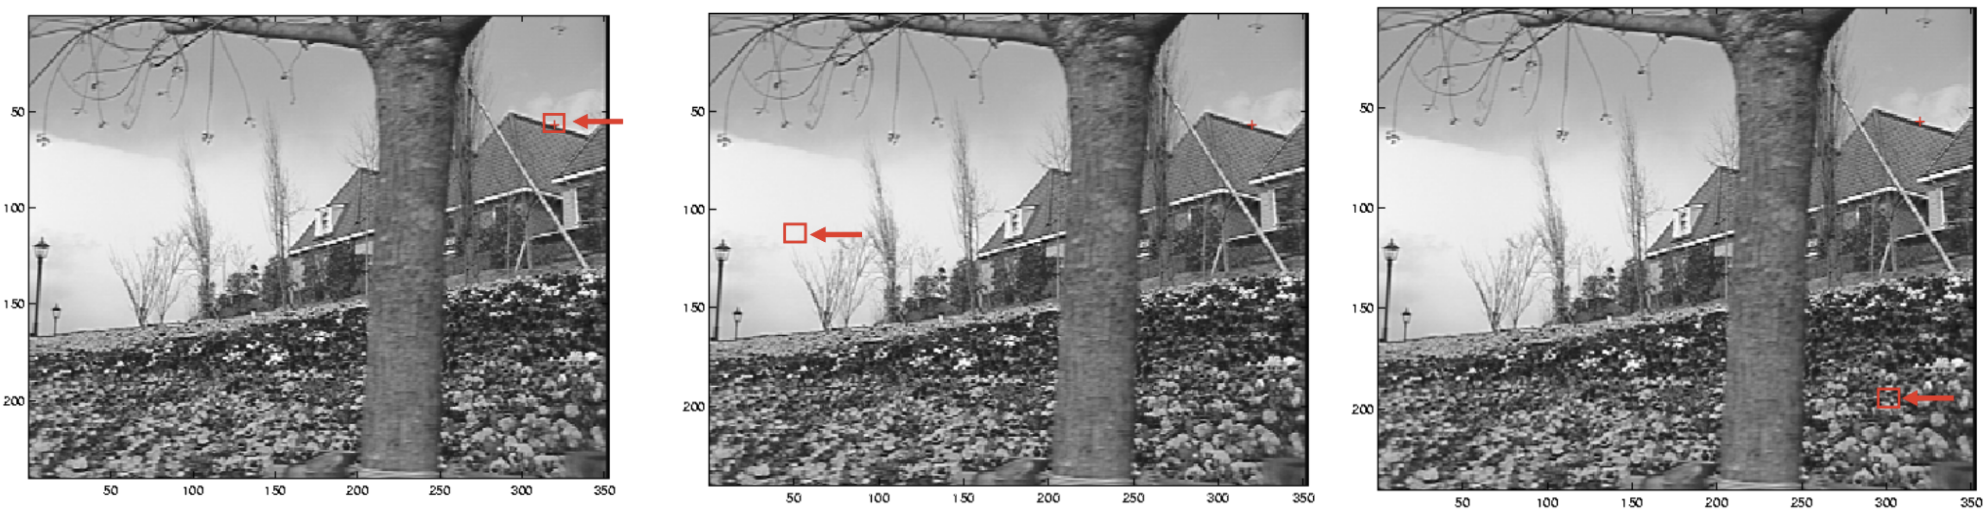
\includegraphics[width=\textwidth]{lk_regions.png}
\caption{Example of regions with large $\lambda_1$ and small $\lambda_2$ (left), small $\lambda_1$ and small$\lambda_2$ (center, low texture region), large $\lambda_1$ and large $\lambda_2$ (right, high texure region)}
\end{figure}

\subsection{Error in Lucas-Kanade}
The Lucas-Kanade method is constrained under the assumptions of optical flow. Supposing that $A^TA$ is easily invertible and that there is not much noise in the image, errors may still arise when:
\begin{itemize}
\item Brightness constancy is not satisfied, meaning that a pixel may change intensity from different time steps.
\item The motion is not small or and does not change gradually over time.
\item Spatial coherence is not  satisfied, meaning neighboring pixels do not move alike.
\subitem This may arise due to in an inappropriately sized window (choosing bad $k$).
\end{itemize}

\subsection{Improving Accuracy}
From the many assumptions made above, Lucas-Kanade can improve its accuracy by including the higher order terms previously dropped in the Taylor expansion approximation for the brightness constancy equation. This loosens the assumptions of small motion and more accurately reflects optical flow. Now, the problem to be solved is:

\[ I(x+u, y+v) = I(x,y) + I_xu + I_yv + \text{higher order terms} - I_{t-1}(x,y)\]

This is a polynomial root finding problem and can be solved with an iterative approach using Newton’s method. 

In summary, the refined Iterative Lucas-Kanade Algorithm may be applied as:
\begin{enumerate}
\item Estimate velocity at each pixel by solving Lucas-Kanade equations.
\item Warp $I(t-1)$ towards $I(t)$ using the estimated flow field and image warping techniques.
\item Repeat until convergence.
\end{enumerate}


\section{Horn-Schunk}

\subsection{Horn-Schunk Method for Optical Flow}
The Horn-Schunk method for computing optical flow formulates flow as the following global energy function which should be minimized with respect to $u(x,y)$ and $v(x,y)$.
\[E=\int\int[(I_xu+I_yv+I_t)^2+\alpha^2(||\nabla u||^2+||\nabla v||^2)]\mathrm{d}x \mathrm{d}y\]
The first term of this energy function reflects the brightness constancy assumption, which states that the brightness of each pixel remains the same between frames, though the location of the pixel may change. According to this assumption, $I_xu+I_yv+I_t$ should be zero. The square of this value is included in the energy function to ensure that this value is as close to zero as possible, and thus $u$ and $v$ comply with the brightness constancy assumption.

The second term of this energy function reflects the small motion assumption, which states that the points move by small amounts between frames. The squares of the magnitudes of $u$ and $v$ are included in the energy function to encourage smoother flow with only small changes to the position of each point. The regularization constant $\alpha$ is included to control smoothness, with larger values of $\alpha$ leading to smoother flow.

To minimize the energy function, we take the derivative with respect to $u$ and $v$ and set to zero. This yields the following two equations
\[I_x(I_xu+I_yv+I_t)-\alpha^2\Delta u=0\]
\[I_y(I_xu+I_yv+I_t)-\alpha^2\Delta v=0\]
where $\Delta=\frac{\partial^2}{\partial x^2}+\frac{\partial^2}{\partial y^2}$ is called the Lagrange operator, which in practice is computed as
\[\Delta u(x,y)=\bar{u}(x,y)-u(x,y)\]
where $\bar{u}(x,y)$ is the weighted average of $u$ in a neighborhood around $(x,y)$. Substituting this expression for the Lagrangian in the two equations above yields
\[(I_x^2+\alpha^2)u+I_xI_yv=\alpha^2\bar{u}-I_xI_t\]
\[I_xI_yu+(I_y^2+\alpha^2)v=\alpha^2\bar{v}-I_yI_t\]
which is a linear equation in $u$ and $v$ for each pixel. 

\subsection{Iterative Horn-Schunk}

Since the solution for $u$ and $v$ for each pixel $(x,y)$ depends on the optical flow values in a neighborhood around $(x,y)$, to obtain accurate values for $u$ and $v$ we must recalculate $u$ and $v$ iteratively once the neighbors have been updated. We can iteratively solve for $u$ and $v$ using
\[u^{k+1}=\bar{u}^k-\frac{I_x(I_x\bar{u}^k+I_y\bar{v}^k+I_t)}{\alpha^2+I_x^2+I_y^2}\]
\[v^{k+1}=\bar{v}^k-\frac{I_y(I_x\bar{u}^k+I_y\bar{v}^k+I_t)}{\alpha^2+I_x^2+I_y^2}\]
where $\bar{u}^k$ and $\bar{v}^k$ are the values for $\bar{u}$ and $\bar{v}$ calculated during the $k$'th iteration, and $u^{k+1}$ and $v^{k+1}$ are the updated values for $u$ and $v$ for the next iteration.

% I'm still somewhat confused about these last two sections, so if someone else can elaborate here that would probably be good
\subsection{Smoothness Regularization}

The smoothness regularization term $||\nabla u||^2+||\nabla v||^2$ in the energy function encourages minimizing change in optical flow between nearby points. With this regularization term, in texture free regions there is no optical flow, and on edges, points will flow to the nearest points, solving the aperture problem.

\subsection{Dense Optical Flow with Michael Black's Method}

Michael Black extended the Horn-Schunk method by replacing the regularization term $||\nabla u||^2+||\nabla v||^2$ which is a quadratic function of the magnitudes of the gradients of $u$ and $v$

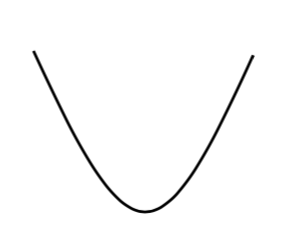
\includegraphics{quadratic.png}

with the following function

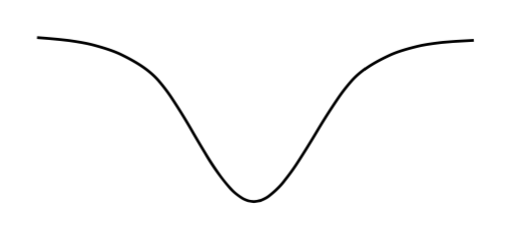
\includegraphics{michaelblack.png}

\section{Pyramids for Large Motion}
Revisiting Lucas-Kanade, recall that one of our original assumptions was that there would be small motion of points between consecutive frames. This assumption causes the algorithm to fall apart when dealing with large motion:

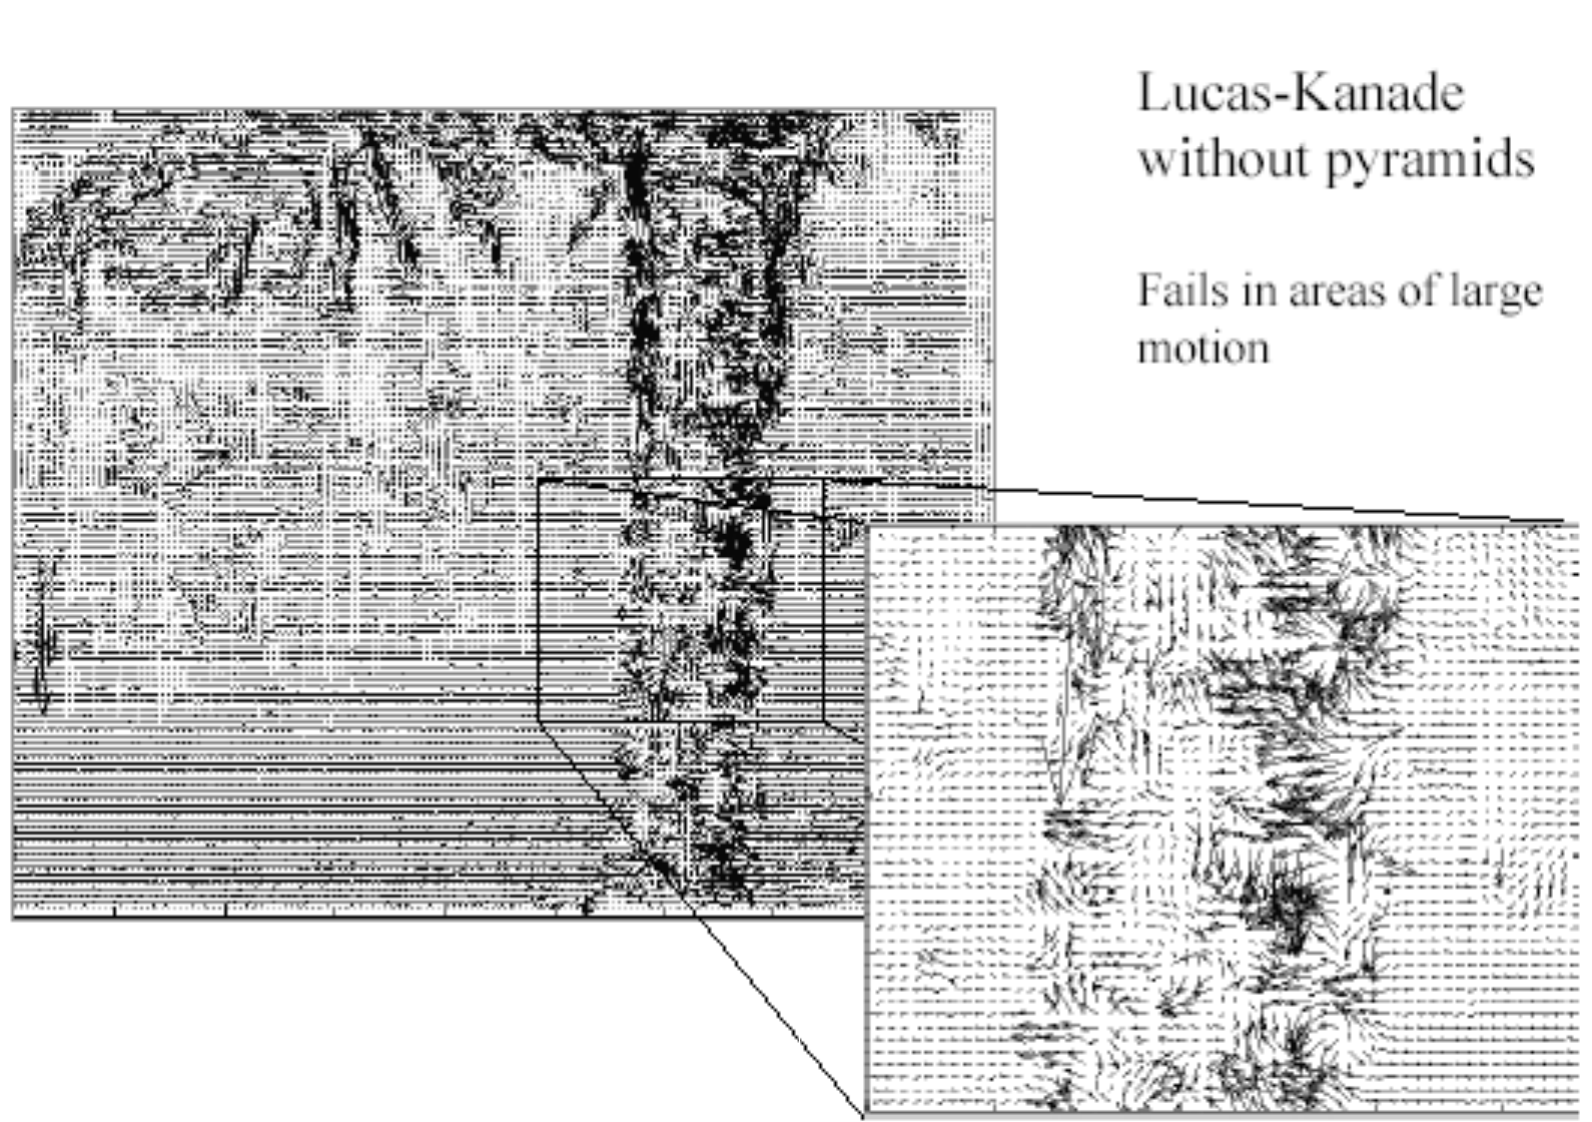
\includegraphics[width=12cm]{wo_pyr.png}

Notice in the graphic above, Lucas-Kanade can't find a consistent vector for the flow of the tree trunk. In order to correct for this, we can apply a tactic where we apply Lucas-Kanade iteratively to a lower-resolution version of the image, similar to how we created image pyramids for our sliding-window feature detector.

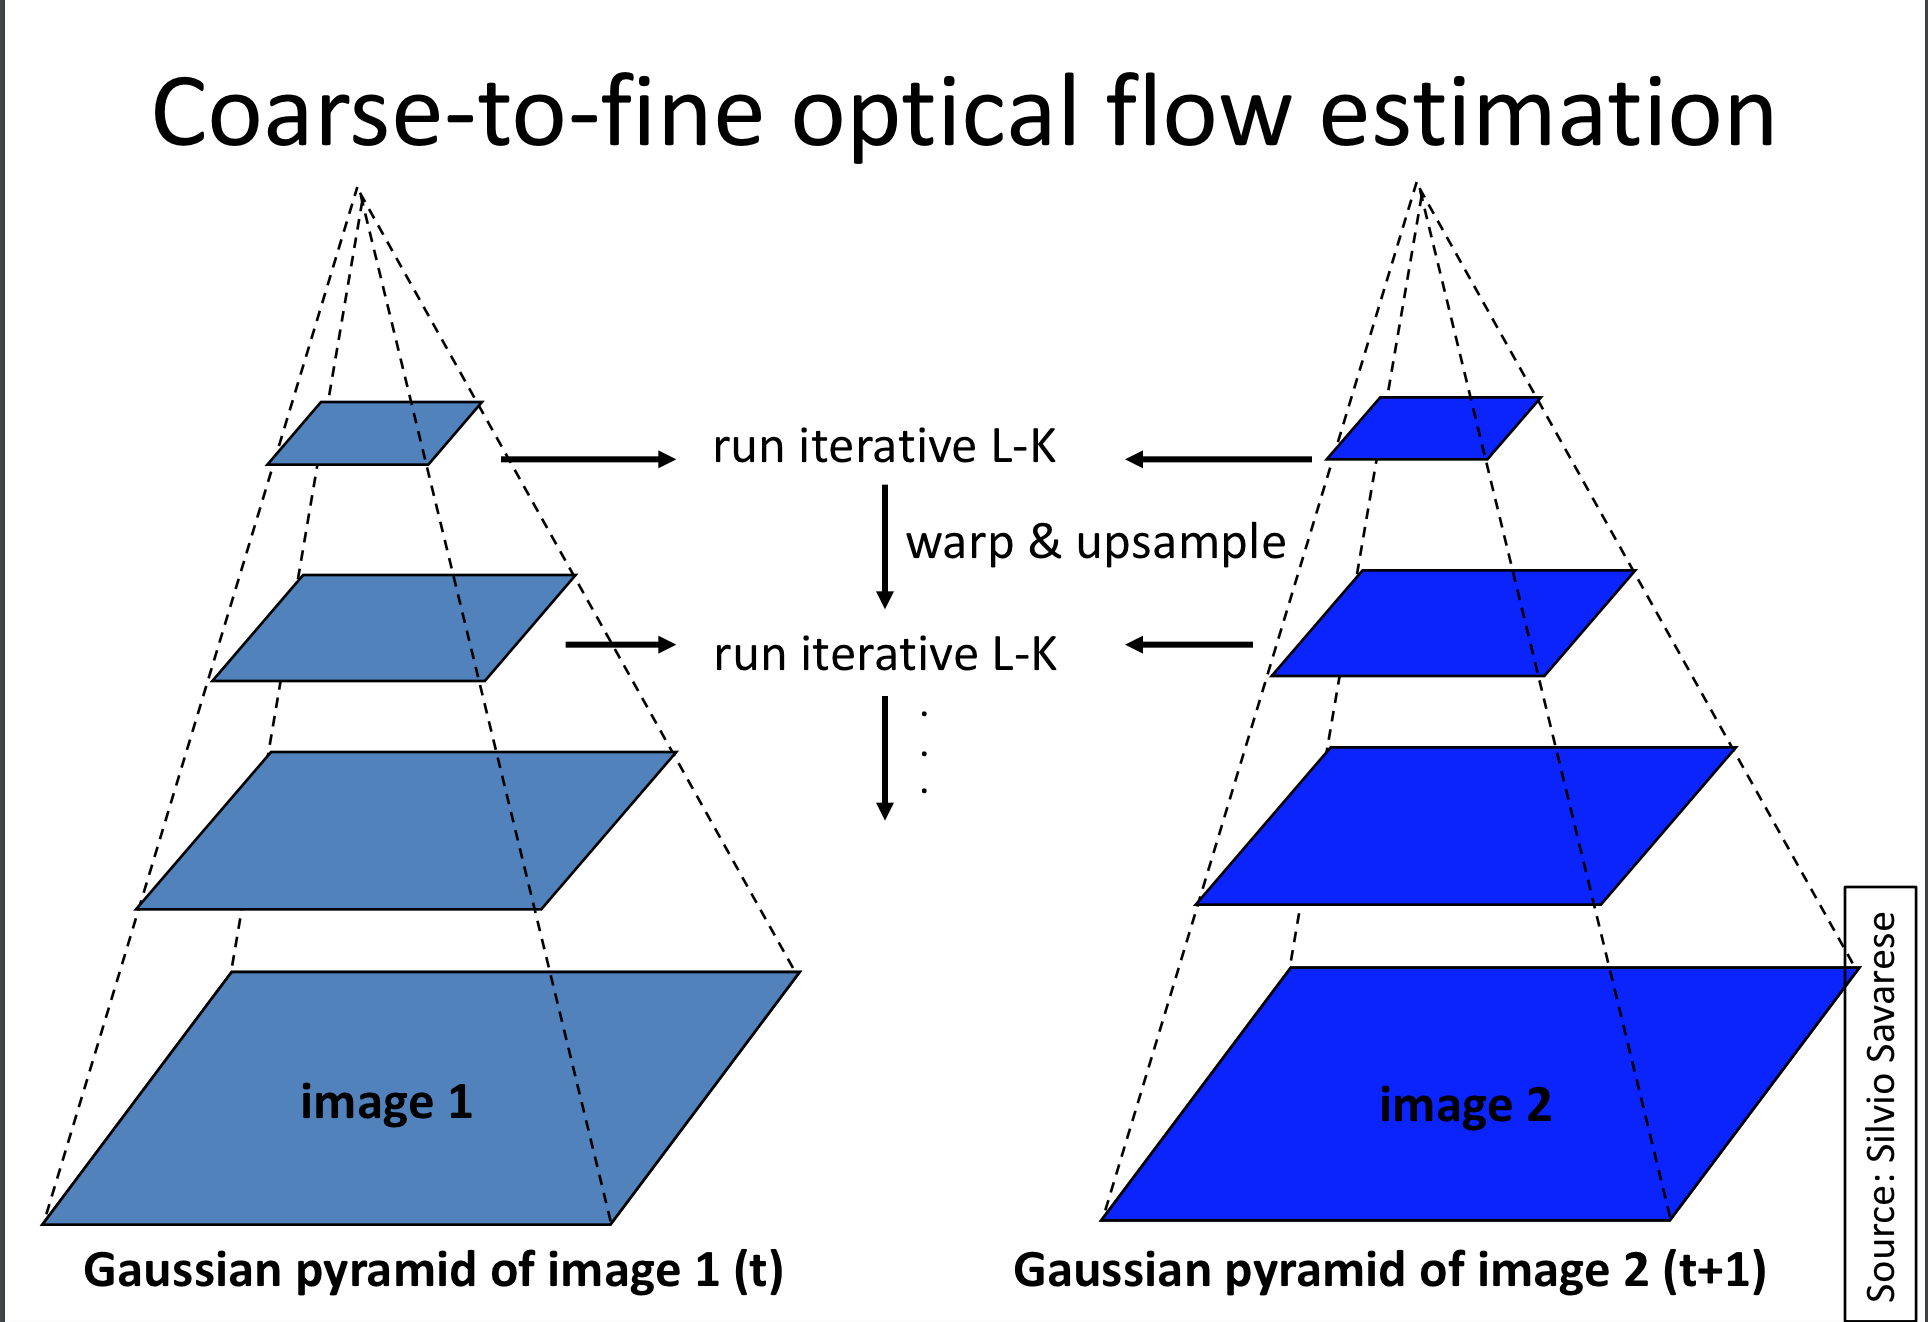
\includegraphics[width=12cm]{lk-pyr.png}

Now, when we try to find the flow vector, the small motion condition is fulfilled, as the downsampled pixels move less from frame to consecutive frame than pixels in the higher resolution image. Here is another example from the slides using Lucas-Kanade with pyramids:

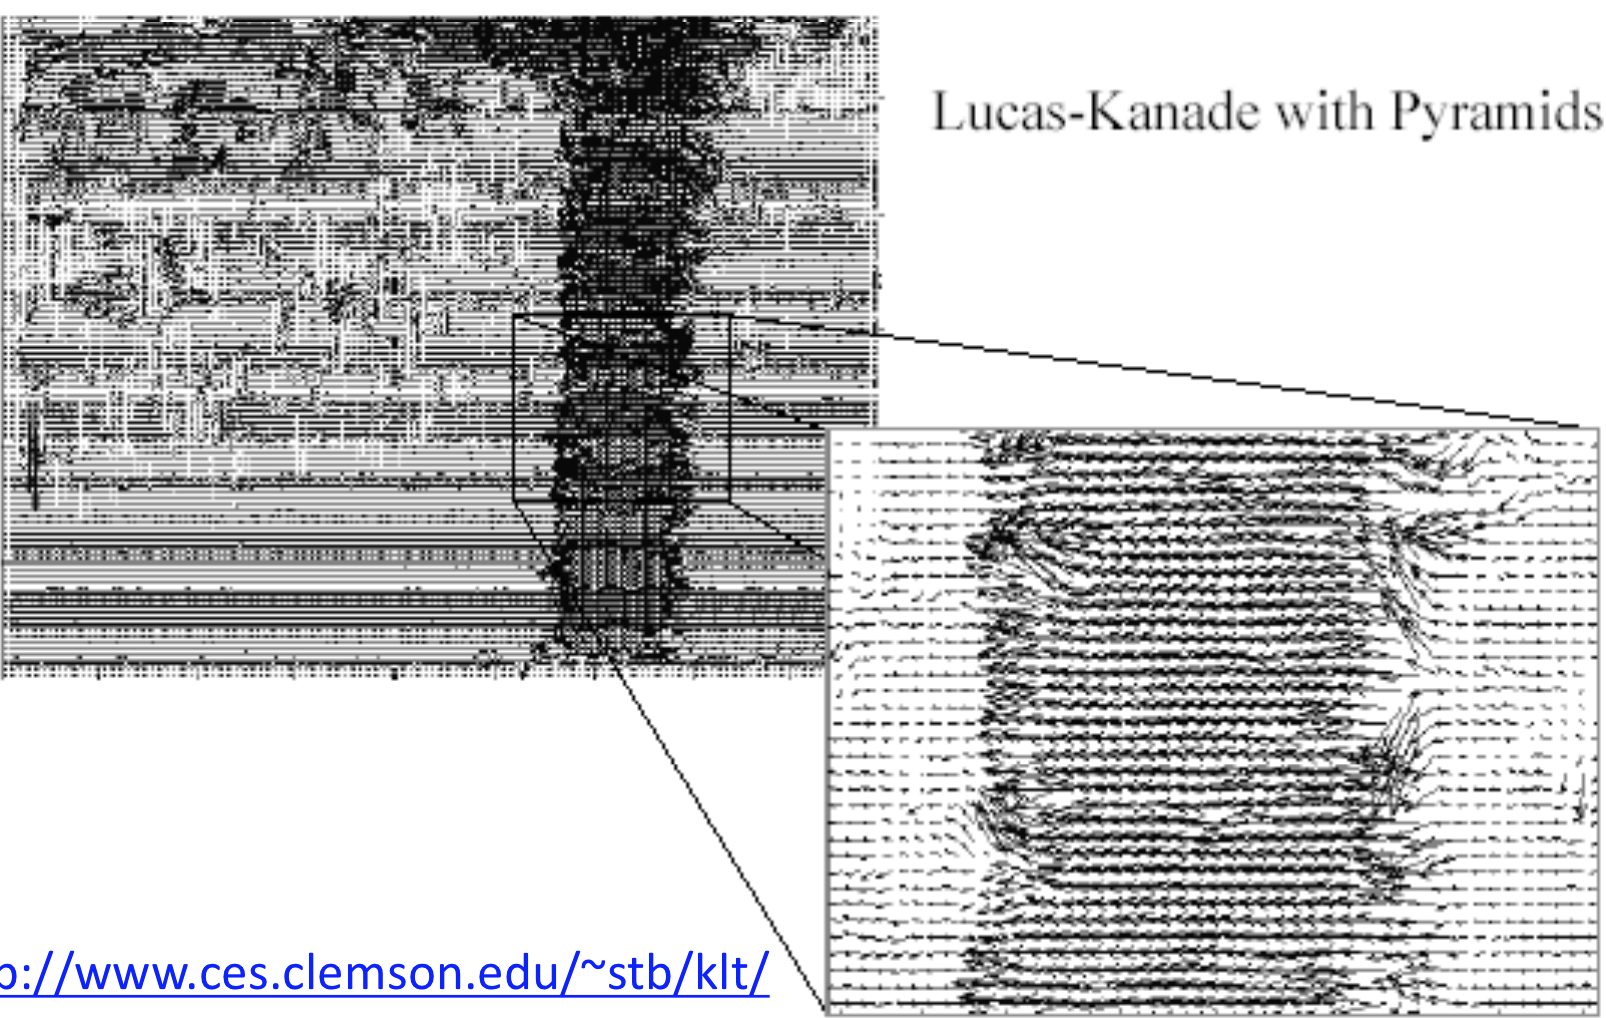
\includegraphics[width=12cm]{w_pyr.png}

Notice how the flow vectors now point mostly in the same direction, indicating that the tree trunk is moving in a consistent direction. 

\section{Common Fate}
We can gain more information about an image by analyzing it through the the lens of common fate, which in this context is the idea that each pixel in a given segment of the image will move in a similar manner. Our goal is to identify the image segments, or "layers", that move together.

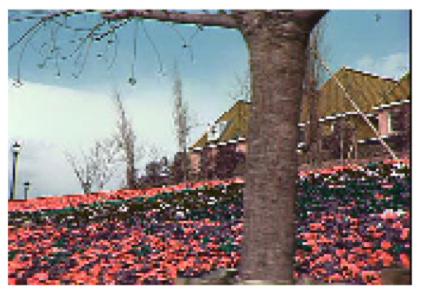
\includegraphics[width=5cm]{treeOriginal.png}
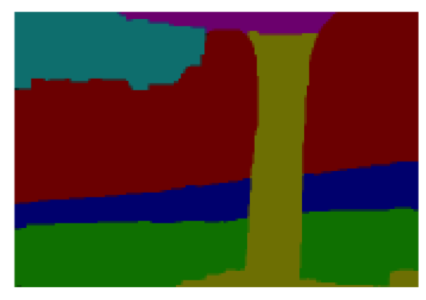
\includegraphics[width=5cm]{treeLayer.png}

\subsection{Identify Layers}
We compute layers in an image by dividing the image into blocks and grouping based on the similarity of their affine motion parameters. For each block, finding the vector $a$ that minimizes
\[Err(a) = \sum[I_x(a_1 + a_2x + a_3y) + I_y(a_4 + a_5x + a_6y) + I_t]^2\]
for all pixels (x, y) in each block.

The above equation is derived from two parts:
(1) the brightness constancy equation, and (2) the components of affine motion:
\[I_xu(x, y) + I_yv(x, y) + I_t \approx 0\]
$I_x, I_y, I_t$ are the gradients of the image with respect to the x direction, y direction, and time, respectively.
$u(x, y)$ and $v(x, y)$ are the components of affine motion in the horizontal and vertical directions:
\[u(x, y) = a_1 + a_2x + a_3y\]
\[v(x, y) = a_4 + a_5x + a_6y\]

From there, we map our parameter vectors $a_i$ into motion parameter space and perform k-means clustering on the affine motion parameter vectors. 

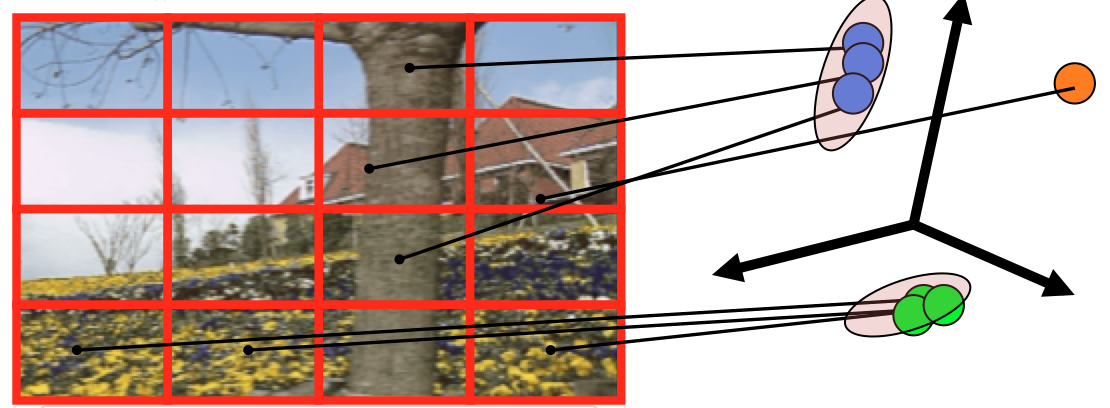
\includegraphics[width=12cm]{grouping.png}


The final centers of the k-means clustering are the parameters $a_1 ... a_6$ that minimize the above error function, and the vectors $a_i$ in each grouping correspond to the original blocks that should be grouped in a single layer. Intuitively, layers should be comprised of blocks that have similar parameters, as that implies their affine motion is similar. 


% References
\small
\bibliographystyle{plain}
\bibliography{bibliography}
% see .bib file fleet2006optical 
% http://www.cs.toronto.edu/~fleet/research/Papers/flowChapter05.pdf
\end{document}
